\section{Preventing Transnational Detours}
\label{avoid_results}

In light of our analysis in Section \ref{datasets}, we now explore how
much techniques and systems can help clients prevent transnational
routing detours. We explore how to (i) increase path diversity with
the use of overlay nodes and (ii) discover additional website replicas
by diverting DNS queries through global open DNS resolvers.  Due to
space limitations, our measurement methods and results on the use of
open DNS resolvers can be found at \cite{characterizing_detours}.
Here, we discuss our measurement method, develop an avoidance metric
and algorithm, and present our results for the use of overlay nodes to
prevent transnational detours.

\subsection{Measurement Approach}
\label{avoid_pipelines}

%\paragraph{Country Avoidance with Open Resolvers.} If content is
%replicated on servers in different parts of the world, open DNS
%resolvers located 
%around the world may also help clients discover a more diverse set of
%replicas.  

%Figure~\ref{fig:avoidance_resolvers} illustrates our measurement
%approach for this study, which differs slightly from that described in
%Section \ref{pipeline}: instead of using RIPE Atlas probes to query
%local DNS resolvers, we query open DNS resolvers located around the
%world~\cite{open_resolver_list}.  These open DNS resolvers may provide
%different IP addresses in the DNS responses, which represent different
%locations of content replicas. The measurement study in
%Section~\ref{pipeline} used RIPE Atlas probes to traceroute to the IP
%addresses in DNS response; in contrast, for this portion of the study we
%initiate a VPN connection to the client's country and traceroute
%(through the VPN connection) to the IP addresses in the DNS responses
%returned by the open resolvers.

%\begin{figure}[t]
%\centering
%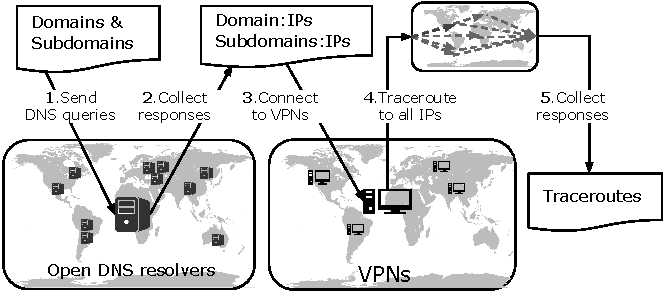
\includegraphics[width=.45\textwidth]{Country-Avoidance-Resolvers}
%\caption{Measurement approach for country avoidance with open DNS resolvers.}
%\label{fig:avoidance_resolvers}
%\end{figure}

%\paragraph{Country Avoidance with Relays.} 
Using an overlay network may
help clients route around unfavorable countries or access content 
that is hosted in a different country.  Figure~\ref{fig:avoidance_relays}
shows the steps to conduct this measurement. 
After selecting relay machines, we run traceroute measurements from
Country X to each relay and from each relay to the set of domains. We
then analyze these traceroutes using the pipeline in Figure
\ref{fig:analysis_pipeline} to determine country-level paths. 

\begin{figure}[t]
\centering
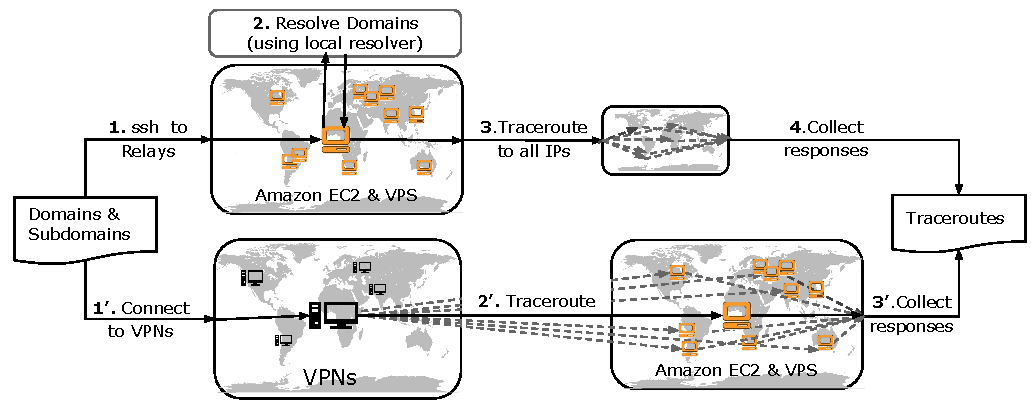
\includegraphics[width=.5\textwidth]{Country-Avoidance-Relays}
\caption{Measurement approach for country avoidance with overlay network relays.}
\label{fig:avoidance_relays}
\end{figure}

We use eight EC2 instances, one in each geographic region
(U.S., Ireland, Germany, Singapore, South Korea, Japan, Australia,
Brazil), as well as four Virtual Private Server (VPS) machines (France,
Spain, Brazil, Singapore), which are virtual machines.
% that are functionally equivalent to dedicated physical servers.  
Combining these two sets of machines allows us to evaluate surveillance avoidance with a geographically diverse set of relays. 
%By selecting an open resolver in each country that also has a relay in it we can keep the variation in measurement methods low, leading to a more accurate comparison of country avoidance methods.

\subsection{Avoidability Metrics}
\label{metrics}

We introduce a new metric and algorithm to measure how often a client in
Country X can avoid a specific country Y.  
%Using the proposed metric
%and algorithm, we can compare how well the different methods achieve
%country avoidance for any (X, Y) pair.

\paragraph{Avoidability metric.}  We introduce an avoidability metric to
quantify how often
traffic can avoid Country Y when it originates in Country X.
Avoidability is the fraction of paths that start in Country
X and do not transit Country Y.  We calculate this value by dividing the
number of paths from Country X to domains that do not traverse Country Y
by the total number of paths from Country X. The resulting value will be
in the range [0,1], where 0 means the country is unavoidable for all of
the domains in our study, and 1 means the client can avoid Country Y for
all domains in our study.  For example, there are three paths
originating in Brazil: (1)~$BR \rightarrow US$, (2)~$BR \rightarrow CO
\rightarrow None$, 3) $BR \rightarrow *** \rightarrow BR$.  After
processing the paths as described in Section \ref{c_map}, the resulting
paths are: (1)~$BR \rightarrow US$, (2)~$BR \rightarrow CO$, (3)~$BR
\rightarrow BR$.  The avoidance value for avoiding the United States
would be 2/3 because two out of the three paths do not traverse the
United States.  This metric represents a lower bound,
because it is possible that the third path timed out ($***$) because it
traversed the United States, which would make the third path: $BR
\rightarrow US \rightarrow BR$, and would cause the avoidance metric to
drop to 1/3.

%\paragraph{Avoidability algorithm with open resolvers.} Recall from the measurement pipeline for avoidance with open resolvers, described in Section \ref{avoid_pipelines}, that the resulting data are traceroutes from the client in Country X to \textit{all} IP addresses in \textit{all} open DNS resolver responses.  To measure avoidability, there must exist at least one path from the client in Country X to the domain for the client to be able to avoid Country Y when accessing the domain.  The country avoidance value is the fraction of domains accessible from the client in Country X without traversing Country Y.

\paragraph{Avoidability algorithm.}  Measuring the avoidability of Country Y from a client in Country X using relays has two components: (1)~Is Country Y on the path from the client in Country X to the relay?  (2)~Is Country Y on the path from the relay to the domain?  For every domain, our algorithm checks if there exists at least one path from the client in Country X through any relay and on to the domain, and does not transit Country Y.  
The algorithm (Algorithm~\ref{avoid_algo}) produces a value in the range
[0,1] that can be compared to the output of the avoidability metric.

\begin{algorithm}[t]
\caption{Avoidability Algorithm}
\label{avoid_algo}
\footnotesize
\begin{algorithmic}[1]
\Function{CalcAvoidance}{set $paths1$, set $paths2$, string c}
    \State set $suitableRelays$
    \For{each $(relay,path)$ in $paths1$} 
    	\If{$c$ not in $path$}
		\State $suitableRelays \gets path$
	\EndIf
    \EndFor
    \State set $accessibleDomains$
    \For{each $(relay,domain,path)$ in $paths2$}
    \If{$relay$ in $suitableRelays$}
        \If{$c$ not in $path$}
        \State $accessibleDomains \gets domain$
        \EndIf
    \EndIf
    \EndFor
    \State $D \gets$ number of all unique domains in $paths2$
    \State $A \gets$ length of $accessibleDomains$
    \State \Return $A / D$
\EndFunction
\end{algorithmic}
\end{algorithm}


\paragraph{Upper bound on avoidability.}  Although the avoidability
metric provides a way to quantify how avoidable Country
Y is for a client in Country X, some
domains may be hosted only in Country Y, so the avoidance value 
would never reach 1.0.  For this reason, we measured the {\em upper
bound} on avoidance for a given pair of (Country X, Country Y) that
represents the best case value for avoidance.  The algorithm analyzes the destinations of all domains from all relays and if there exists at least one destination for a domain that is not in Country Y, then this increases the upper bound value.  An upper bound value of 1.0 means that every domain studied is hosted (or has a replica) outside of Country Y.  This value puts the avoidance values in perspective for each (Country X, Country Y) pair. 

%\begin{algorithm}[t]
%\caption{Avoidance Upper Bound Algorithm}
%\label{upperbound_algo}
%\small
%\begin{algorithmic}[1]
%\Function{CalcUpperbound}{set $relayDomainPaths$, string $c$}
%    \State $zeros(domainLocations)$
%    \For{each $(r,d,p)$ in $relayDomainPaths$} 
%		\State $dest \gets $ last item in $p$
%		\State $domainLocations[d] \gets dest$
%    \EndFor
%    \State set $accessibleDomains$
%    \For{each $domain$ in $domainLocations$}
%    \If{$domainLocations[domain] \neq $ set[$c$]}
%    \State $accessibleDomains \gets domain$
%    \EndIf
%    \EndFor
%    \State $D \gets$ all unique domains in  $relayDomainPaths$
%    \State $A \gets$ length of $accessibleDomains$
%    \State \Return $A / D$
%\EndFunction
%\end{algorithmic}
%\end{algorithm}

\subsection{Results}

We examine the
effectiveness of relays for country avoidance, as well as for keeping local
traffic local.  Table \ref{tab:avoid} shows avoidance values; the top
row shows the countries we studied and the left column shows the country
that the client aims to avoid.
%
As seen in Table \ref{tab:avoid}, there are two significant trends: 1) the ability for a client to avoid a given Country Y increases with the use of relays, and 2) the least avoidable countries are surveillance states. 

%\newcolumntype{d}[1]{D{.}{.}{#1}}
\begin{table*}[t]
\tiny
\centering
\resizebox{\textwidth}{!}{%
\begin{tabular}{P{32mm}|d{3.2}d{3.2}|d{3.2}d{3.2}|d{3.2}d{3.2}|d{3.2}d{3.2}|d{3.2}d{3.2}}
\multicolumn{1}{l}{}    & \headrow{No Relay} & \headrow{Relays} & \headrow{No Relay}  & \headrow{Relays} & \headrow{No Relay}  & \headrow{Relays}   & \headrow{No Relay}  & \headrow{Relays}  & \headrow{No Relay} & \headrow{Relays} \\ \toprule
\textit{Country to Avoid}    &\multicolumn{2}{c|}{\textit{Brazil}}   &\multicolumn{2}{c|}{\textit{Netherlands}}   &\multicolumn{2}{c|}{\textit{India}} &\multicolumn{2}{c|}{\textit{Kenya}} &\multicolumn{2}{c}{\textit{United States}}\\ \toprule

Brazil               &0.00     &0.00     &1.00  &1.00   &1.00    &1.00   &1.00  &1.00  &1.00  &1.00  \\ \midrule
Canada               &.98    &1.00     &.99 &1.00   &.98  &.98  &.99  &.99  &.92  &1.00  \\
United States        &\cellcolor[HTML]{F7BE81}.15  &\cellcolor[HTML]{F7BE81}.62     &\cellcolor[HTML]{F7BE81}.41 &\cellcolor[HTML]{F7BE81}.63   &\cellcolor[HTML]{F7BE81}.28  &\cellcolor[HTML]{F7BE81}.65  &\cellcolor[HTML]{F7BE81}.38  &\cellcolor[HTML]{F7BE81}.40  &\cellcolor[HTML]{F7BE81}0.00 &\cellcolor[HTML]{F7BE81}0.00  \\ \midrule
France               &.94  &1.00     &.89 &.99   &.89 &1.00  &.77 &.98  &.89 &.99  \\
Germany              &.99 &1.00     &.95 &.99   &.96  &.99  &.95 &1.00  &.99 &1.00  \\
Great Britain        &.97  &1.00     &.86 &.99   &\cellcolor[HTML]{F7BE81}.79  &\cellcolor[HTML]{F7BE81}1.00  &\cellcolor[HTML]{F7BE81}.50  &\cellcolor[HTML]{F7BE81}.97  &.99 &1.00  \\
Ireland              &.97  &.99     &.89 &.99   &.96 &.99  &.86 &.99  &.99 &.99  \\
Netherlands          &.98  &.99     &0.00 &0.00   &.87  &.99  &\cellcolor[HTML]{F7BE81}.74  &\cellcolor[HTML]{F7BE81}.99  &.97 &.99  \\
Spain                &.82  &1.00     &.99 &.99   &1.00  &1.00  &1.00  &1.00  &1.00 &1.00  \\ \midrule
Kenya                &1.00  &1.00     &1.00 &1.00   &1.00  &1.00  &0.00 &0.00  &1.00 &1.00  \\
Mauritius            &1.00  &1.00     &1.00 &1.00   &1.00  &1.00  &\cellcolor[HTML]{F7BE81}.67 &\cellcolor[HTML]{F7BE81}.99  &1.00 &1.00  \\
South Africa         &1.00  &1.00     &1.00 &1.00   &1.00 &1.00  &\cellcolor[HTML]{F7BE81}.66 &\cellcolor[HTML]{F7BE81}.66  &1.00 &1.00  \\ \midrule
United Arab Emirates &1.00  &1.00     &1.00 &1.00   &1.00 &1.00  &\cellcolor[HTML]{F7BE81}.84 &\cellcolor[HTML]{F7BE81}.99  &1.00 &1.00  \\
India                &1.00  &1.00     &.99 &1.00   &0.00 &0.00  &.94 &1.00  &.99 &1.00  \\
Singapore            &.99  &1.00     &.99 &1.00   &\cellcolor[HTML]{F7BE81}.73  &\cellcolor[HTML]{F7BE81}.94  &.96 &1.00  &.99 &1.00  \\\midrule
\end{tabular}
}
\caption{Avoidance values for different country-avoidance techniques.  The upper bound on avoidance is 1.0 in most cases, but not all.  It is 
common for some European countries to host a domain, and therefore the upper bound is slightly lower than 1.0.  The upper bound on avoidance of the 
U.S. is significantly lower than for any other country; .886, .790, .844, and .765 are the upper bounds on avoidance 
of the U.S. for paths originating in Brazil, Netherlands, India, and Kenya, respectively.}
\label{tab:avoid}
\end{table*}

%\subsubsection{Avoidance with Open Resolvers}

%A given country is more avoidable (higher avoidance value) when open
%resolvers are used as a tool for country avoidance. 

%\begin{finding}[Open Resolver Effectiveness]
%Using open DNS resolvers for country avoidance achieves more country
%avoidance than using local resolvers and less (or equal)
%avoidance than using relays for clients in most
%countries. 
%\end{finding}
%\noindent
%For Brazilian paths, open resolvers only achieve 4\% more avoidance than
%using local resolvers when avoiding the United States, whereas relays
%achieve 47\% more avoidance.  On the other hand, open resolvers are
%about as effective as relays are for avoidance for paths originating in
%the United States.   

%\begin{finding}[Kenya as an Outlier]
%For clients in Kenya, open DNS resolvers are significantly more
%effective than relays for 
%avoiding the United States, South Africa, and the United Arab Emirates.
%\end{finding}
%\noindent
%Clients in Kenya should use open DNS resolvers when avoiding specific
%countries, as they can avoid these specific countries more often than
%when using relays.  Kenyan clients can avoid the United States for 55\%
%of paths when using open resolvers, whereas they can only avoid the United States for 40\% of
%paths when using relays.  The difference in how often the United States can be avoided can be
%attributed to the lower amount of DNS diversity when using relays as
%compared to using open resolvers. For a client in Kenya trying to avoid
%the United States, the client can only use the relay located in Ireland
%(because all paths from the client to the other relays traverse the
%United States), and therefore only gets DNS responses from locally
%resolving domains on the Ireland relay.  When using open resolvers, the
%client gets more DNS diversity as he gets DNS responses from all open
%resolvers located in different countries. 

%The amount of avoidance Kenyan clients can achieve for avoiding South Africa is the same,
%regardless of whether the client is using relays, because all paths
%between the client and the relays traverse South Africa.  Fortunately,
%clients can avoid South Africa for significantly more paths when using
%open resolvers, likely as a result of the fact that open DNS resolvers
%can better uncover hosting diversity.   

%\subsubsection{Avoidance with Relays}
\begin{finding}[Relay Effectiveness]
For 84\% of the (Country X, Country Y) pairs shown in Table \ref{tab:avoid} the avoidance with relays reaches the upper bound on avoidance. 
\end{finding}
\noindent
In almost every (Country X, Country Y) pair, where Country X is the
client's country (Brazil, Netherlands, India, Kenya, or the United
States) and Country Y is the country to avoid, the use of an overlay
network makes Country Y more avoidable than the default routes.  The one
exception we encountered is when a client is located in Kenya and wants
to avoid South Africa, where, as mentioned, all paths through our
relays exit Kenya via South Africa.

\begin{finding}[Relays Achieve Upper Bound]
Clients in the U.S. can achieve the upper bound of avoidance for all
countries---relays help clients in
the U.S. avoid all other Country Y unless the domain is hosted in Country~Y.  
\end{finding}
\noindent
Relays are most effective for clients in the United States.  On the other hand, it is much rarer for (Kenya, Country Y) pairs to achieve the upper bound of surveillance, showing that it is more difficult for Kenyan clients to avoid a given country.  This is not to say that relays are not effective for clients in Kenya; for example, the default routes to the top 100 domains for Kenyans avoid Great Britain 50\% of the time, but with relays this percentage increases to about 97\% of the time, and the upper bound is about 98\%. 
%Figure \ref{fig:ke_avoidance} shows default avoidance, avoidance with relays, and the upper bound for Kenya; it's clear that despite having the worst position for avoidance out of the studied countries, in most cases the avoidance with relays either reaches or because extremely close to the upper bound.  

\begin{finding}[Surveillance States are Less Avoidable]
The ability for any country to avoid the U.S. is significantly lower than its ability to avoid any other country in all three situations: without relays, with relays, and the upper bound. 
\end{finding}
%Certain surveillance states discussed in Section \ref{surv} are completely unavoidable a small fraction of time from certain client locations.  France is unavoidable for a small percentage of domains for clients located in the Netherlands, Kenya, and the United States.  Similarly, clients in the Netherlands and Kenya cannot avoid Great Britain for a small fraction of domains.  
\noindent
Despite increasing the ability to avoid the U.S., relays are less
effective at avoiding the U.S. compared to all other Country Y.
Clients in India can avoid the U.S. more often than clients in Brazil,
Netherlands, and Kenya, by avoiding the U.S. for 65\% of paths.  Even
using relays, Kenyan clients can only avoid the U.S. 40\% of the time.  Additionally, the upper bound for avoiding the U.S. is significantly lower in comparison to other countries.  

\begin{finding}[Keeping Local Traffic Local]
Using relays decreased both the number of tromboning paths, and the
number of countries involved in tromboning paths.
\end{finding}
\noindent
Where there were relays located in one of the five
studied countries, we evaluated how well the relays kept local
traffic local.  This evaluation was possible for the U.S. and Brazil.
Tromboning Brazilian paths decreased from 13.2\% without relays to
9.7\% with relays; when relays are used, all tromboning paths go only
to the U.S.  With the relays, we see only 1.3\% tromboning paths for a
U.S. client, compared to 11.2\% without relays.  The 1.2\% of
paths that trombones from the U.S. go only to Ireland.

%\subsubsection{Comparing Avoidance Techniques}

%From the results shown in Table \ref{tab:avoid}, we can see that using open DNS resolvers for country avoidance is, for the most part, less effective than using overlay network relays.  Only 4\% of the (origin country, country to avoid)-pairs shown in the table have a higher avoidance value when using open resolvers in comparison to overlay network relays; in reality, this percentage is actually much lower as Table \ref{tab:avoid} is an abbreviated version of the full table (which can be seen at \annie{fill this in}).  For this reason, we design and implement our system, \system{}, solely using overlay network relays (and not open DNS resolvers).  These few instances where relays were less effective could be remedied by increasing the number and/or geographic diversity of the relays, resulting in the open resolvers providing no additional avoidance after the relays.  We discuss the system and the implementation of the relays in further detail in the next few sections.
